\documentclass[compress]{beamer}

\usetheme{Szeged}
\usepackage[T1]{fontenc}
\usepackage[utf8]{inputenc}
\usepackage[frenchb]{babel}
\usepackage[babel=true,kerning=true]{microtype}
\usepackage{tikz,listings,algorithm,algorithmic,hyperref}
\usetikzlibrary{automata,shapes,snakes,arrows}

\tikzstyle{every picture}=[sibling distance=3cm, shorten >=1pt, node distance=2cm,%
	>=stealth', bend angle=10, auto, initial text=]

\title[IENAC S09 - IA]{{\Large Intelligence Artificielle}\\Exemples}
\author[Charles Lesire]{Charles Lesire-Cabaniols (ONERA / DCSD)\\{\tt charles.lesire@onera.fr}}
\date[2010-2011]{3A-SEM - 2010-2011}

\graphicspath{{../figures/},{../figures/projets/}}
\lstset{basicstyle=\tiny,tabsize=2,%frame=single,%
	emph={define,domain,requirements,strips,typing,types,predicates,
		action,parameters,precondition,vars,effect,objects,init,goal},%
	emphstyle=\bf}

\begin{document}

\begin{frame}
\titlepage
\end{frame}

\section{Exemples}

\subsection{Planification}

\begin{frame}{Formule Dé}
\begin{center}
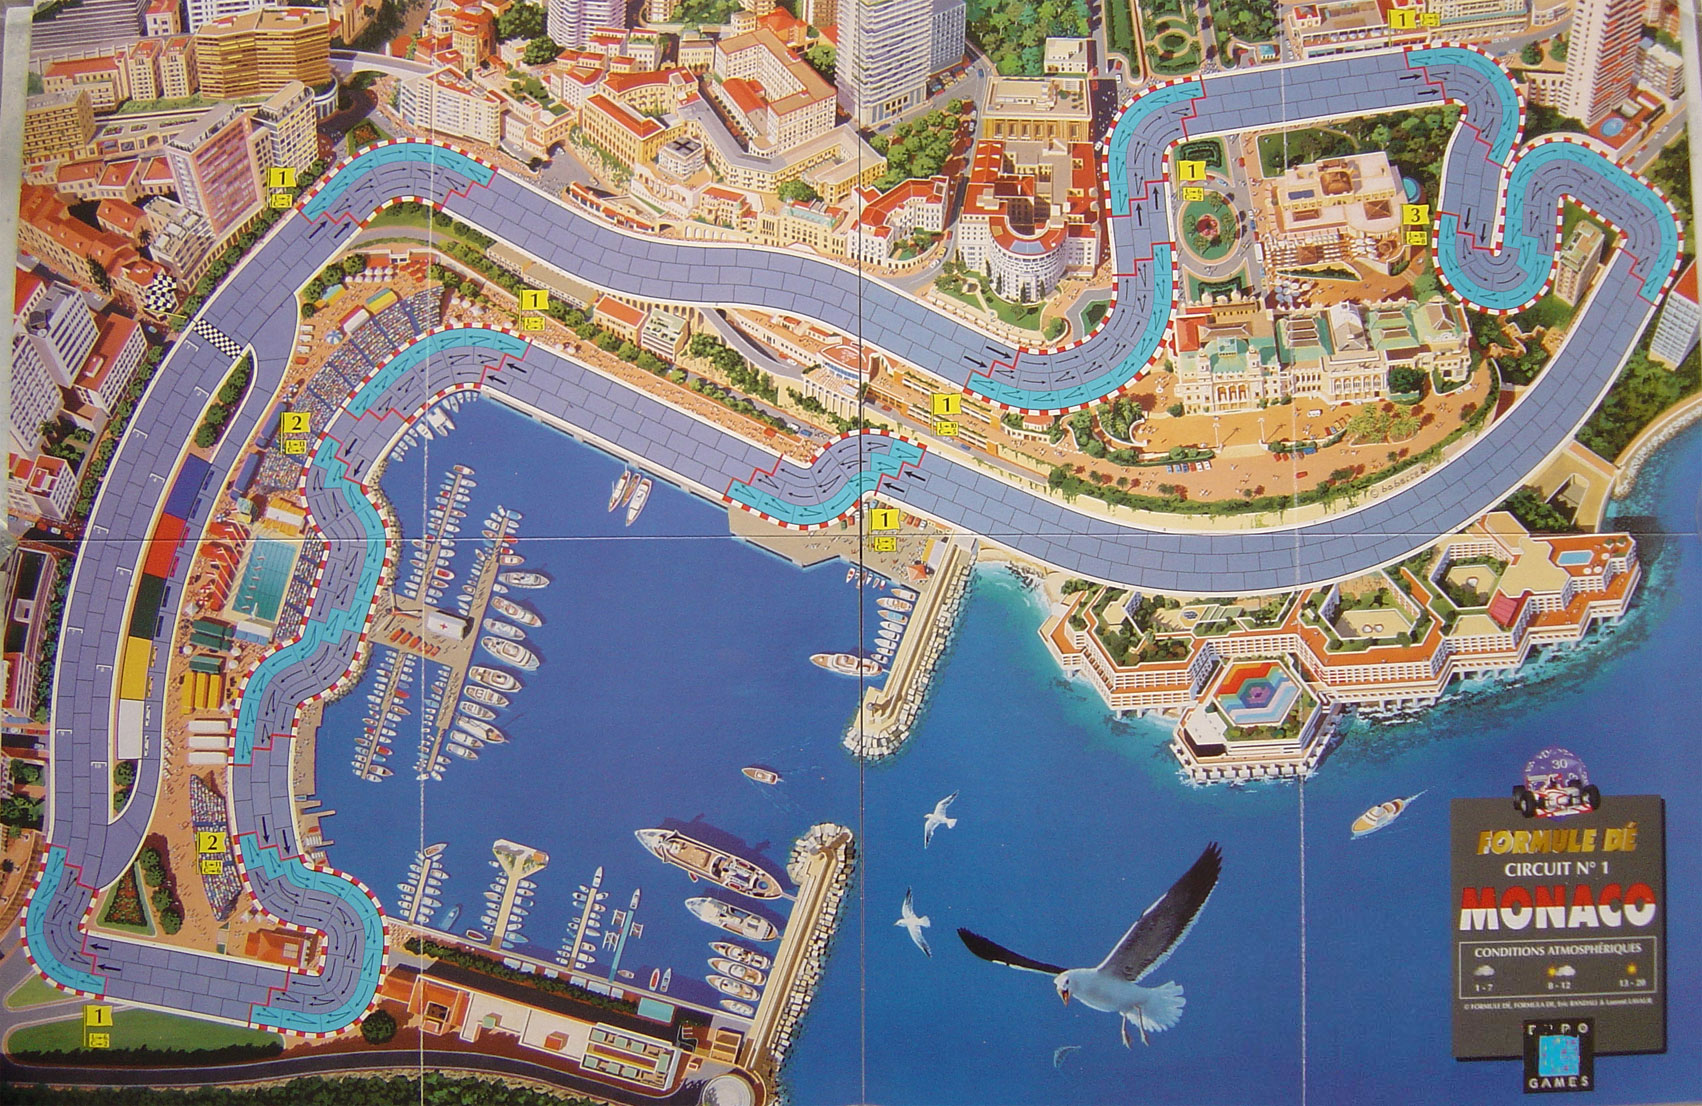
\includegraphics[width=.9\linewidth]{formule_de}
\end{center}
\end{frame}

\begin{frame}{Déplacement en formation}
\begin{center}
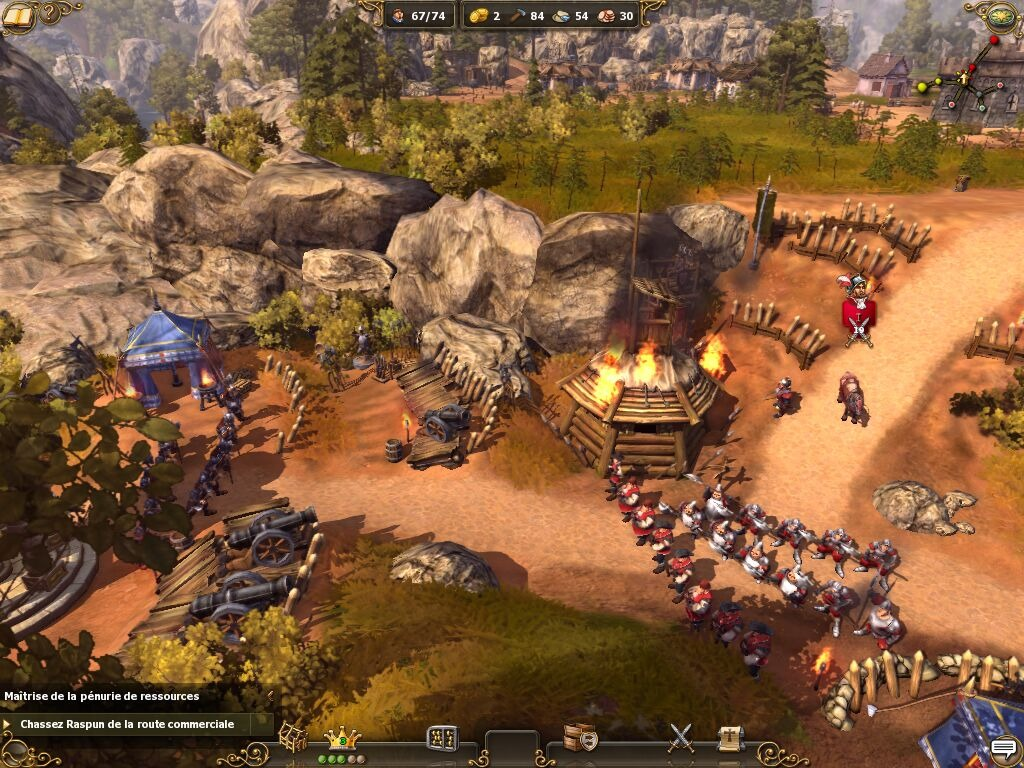
\includegraphics[width=.8\linewidth]{formation}
\end{center}
\end{frame}

\begin{frame}{Planification de trajectoire pour drones}
\begin{center}
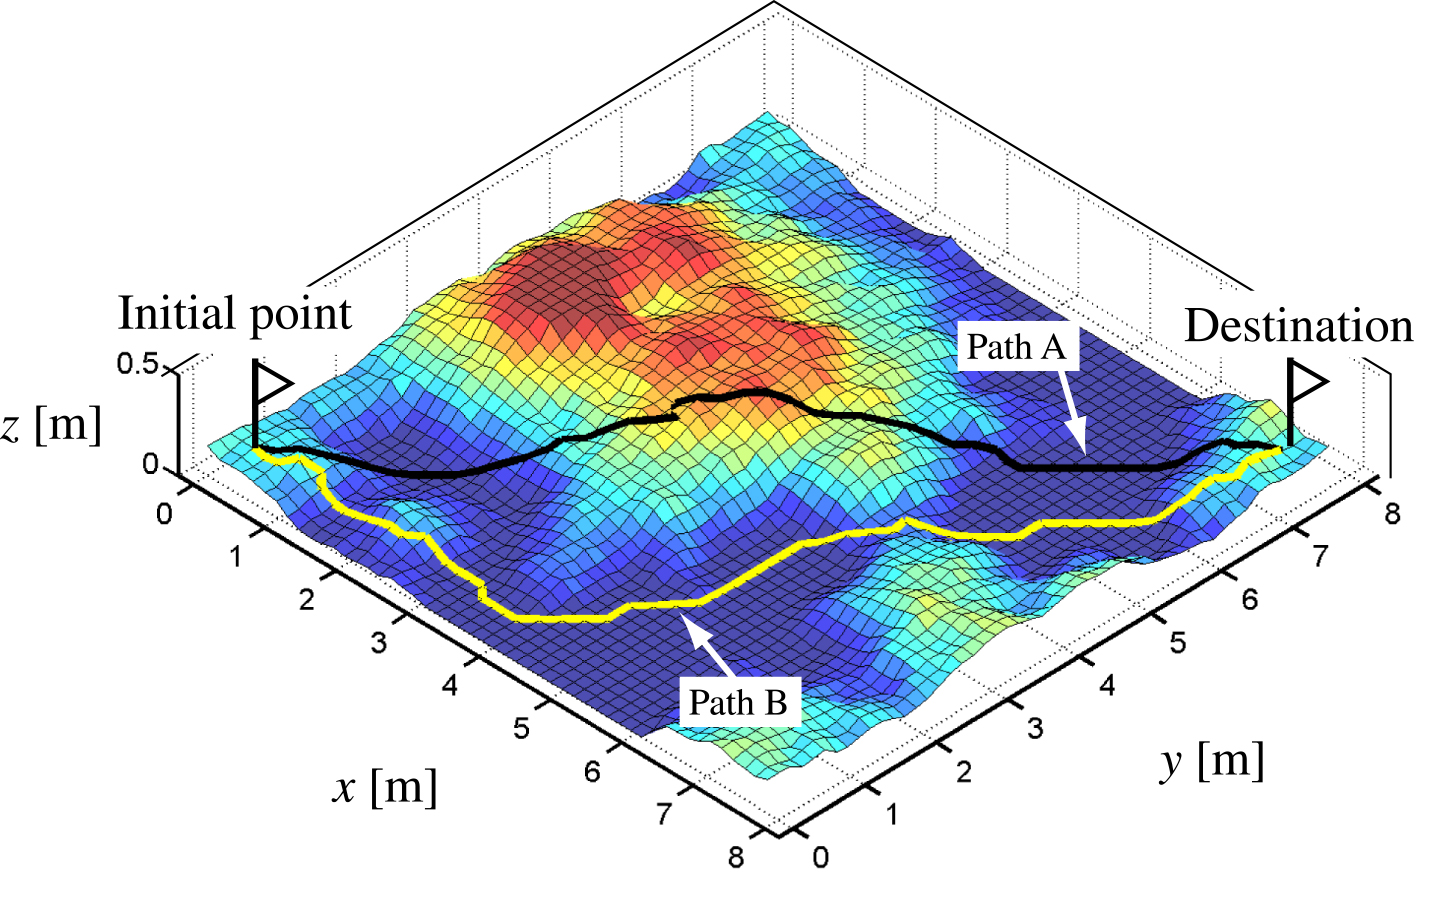
\includegraphics[width=.8\linewidth]{path_planning}
\end{center}
\end{frame}

\begin{frame}{Séquencement de pistes}
\begin{center}
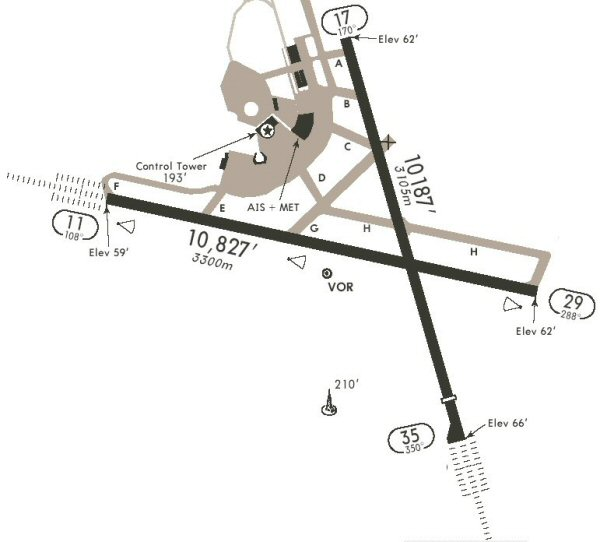
\includegraphics[width=.6\linewidth]{pistes}
\end{center}
\end{frame}

\begin{frame}{Trajectoires de roulage}
\begin{center}
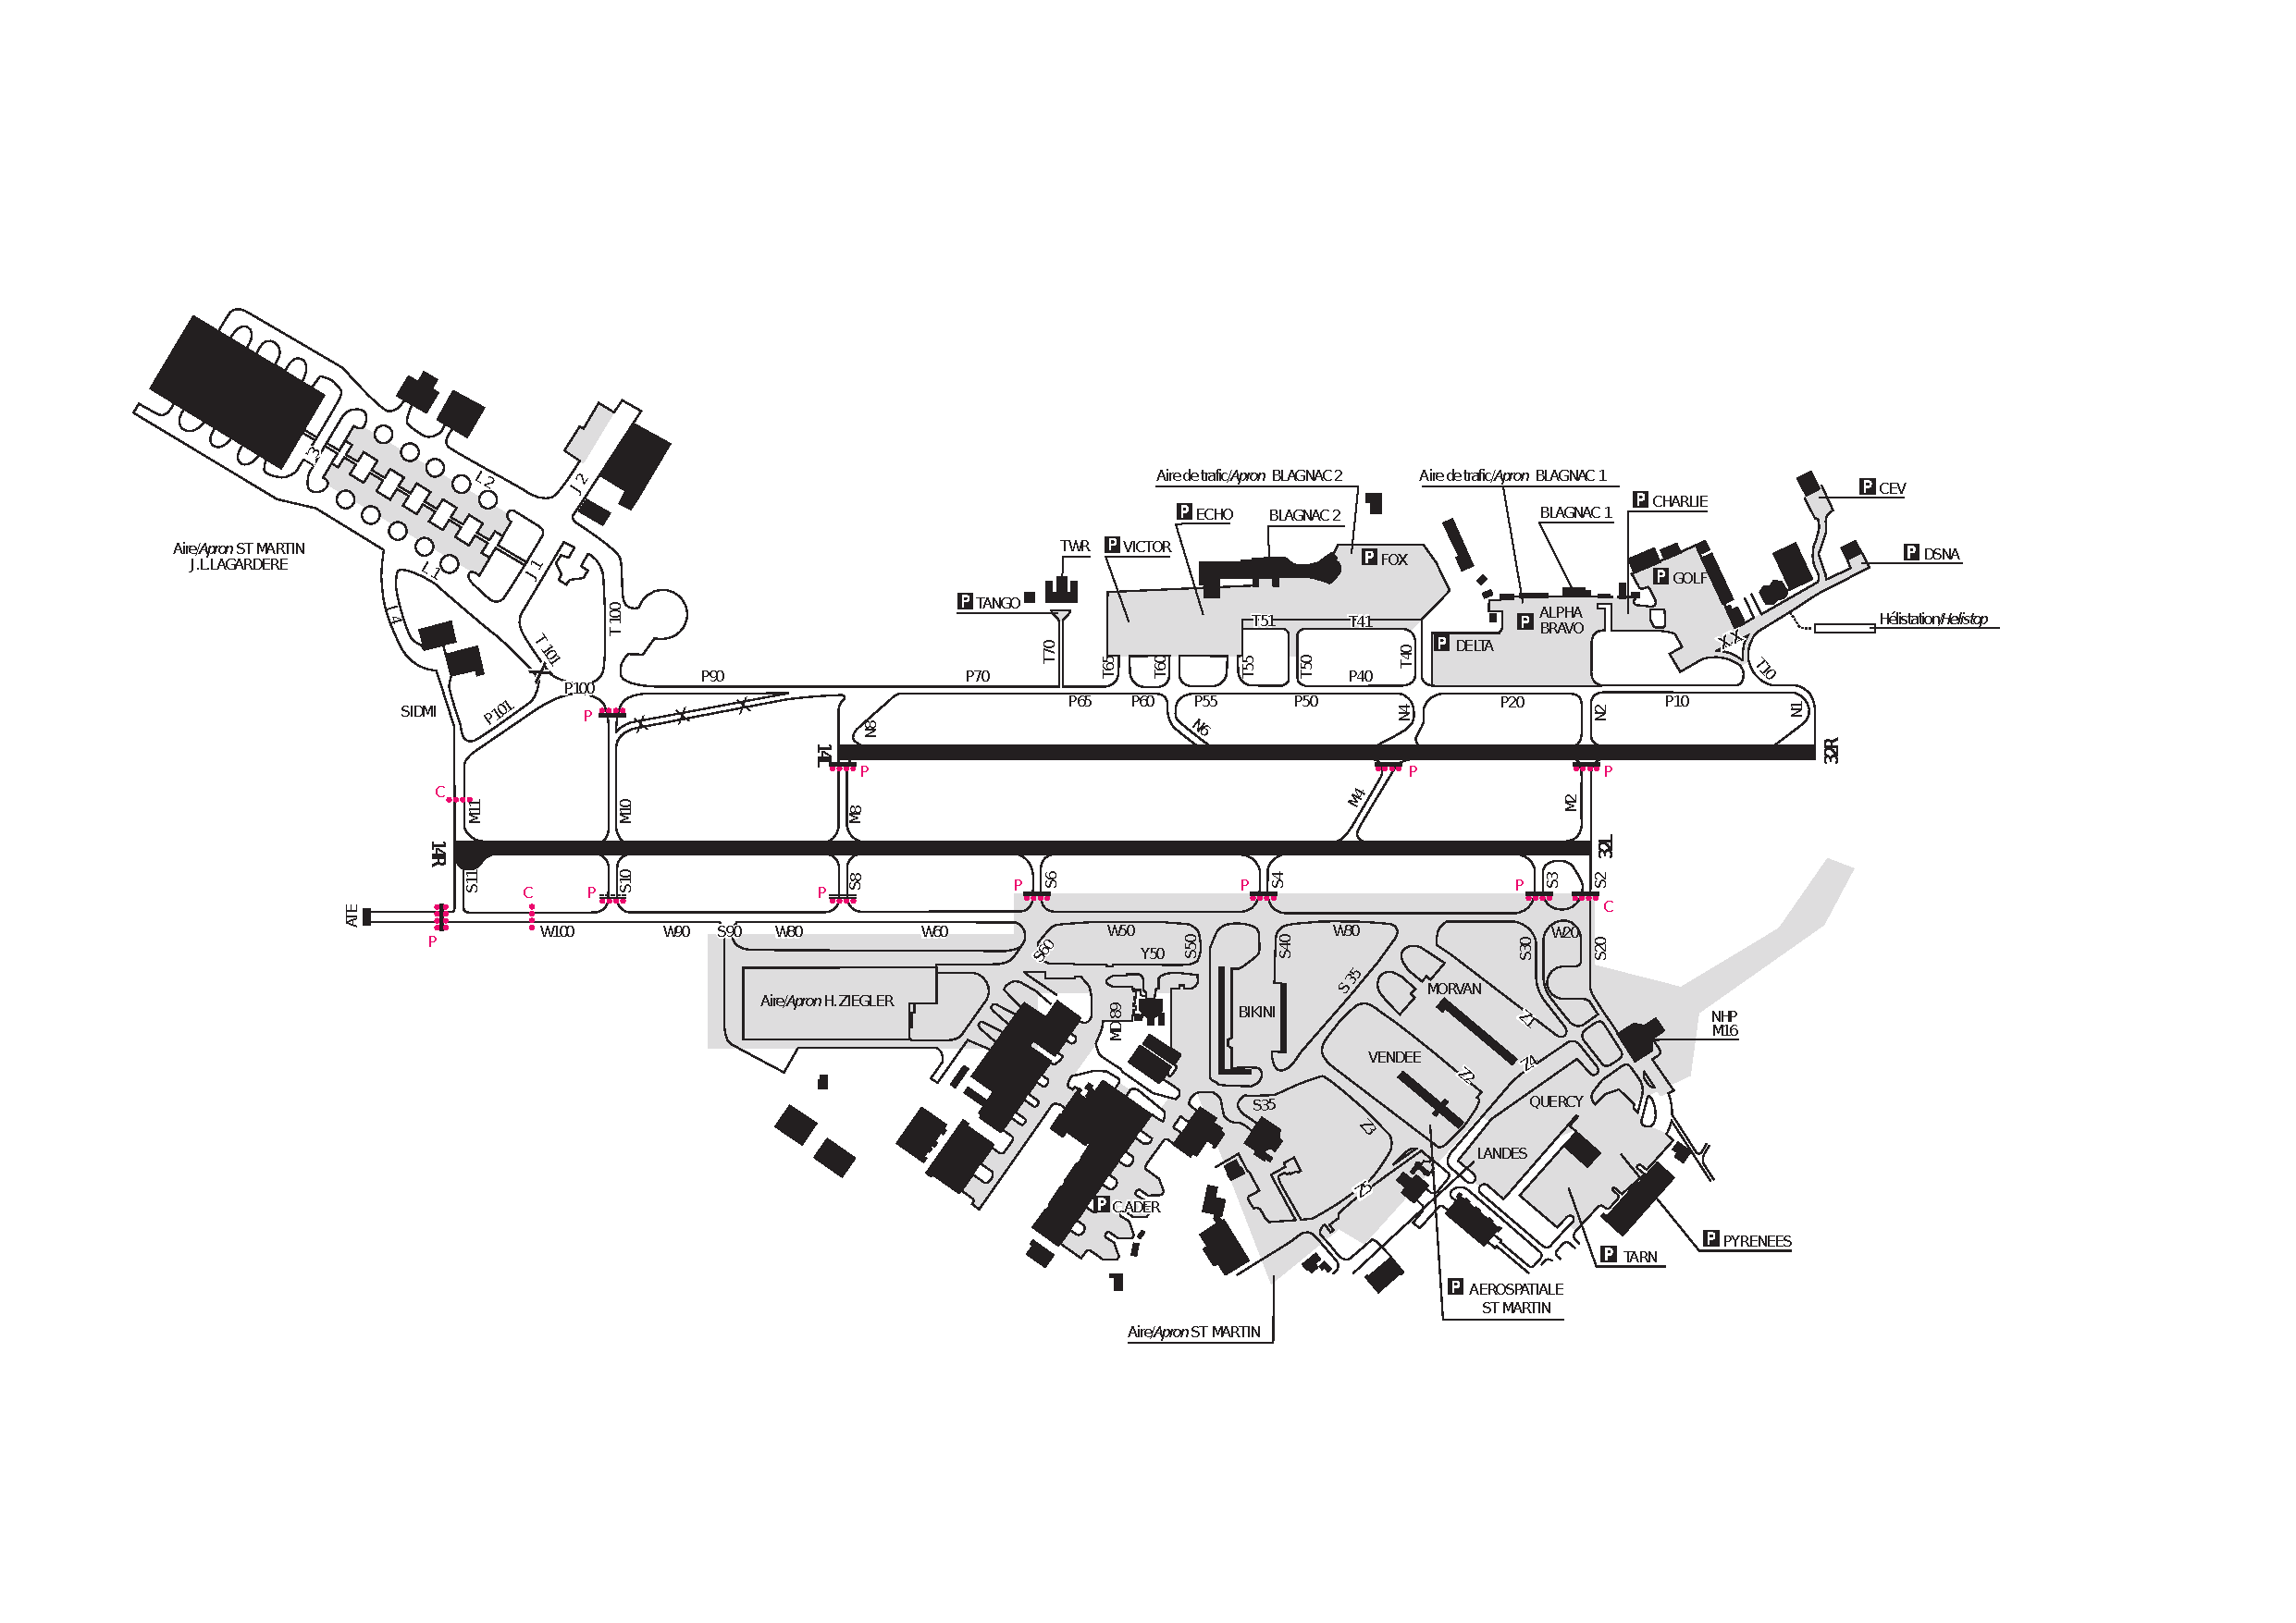
\includegraphics[width=\linewidth]{carte-blagnac}
\end{center}
\end{frame}

\begin{frame}{Ikéa}
\begin{center}
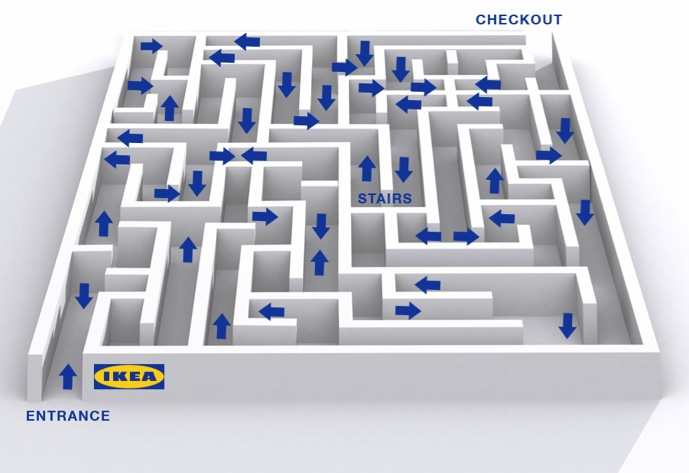
\includegraphics[width=.8\linewidth]{ikea}
\end{center}
\end{frame}

\begin{frame}{Simulation de trafic routier}
\begin{center}
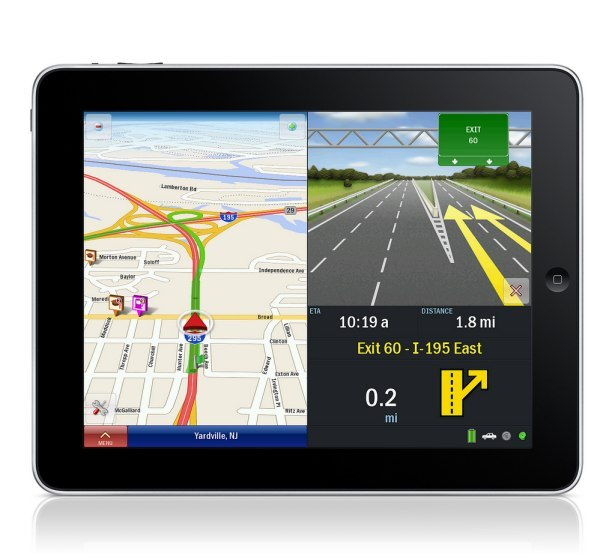
\includegraphics[width=.7\linewidth]{gps}
\end{center}
\end{frame}

\begin{frame}{Concours de Robotique}
\begin{center}
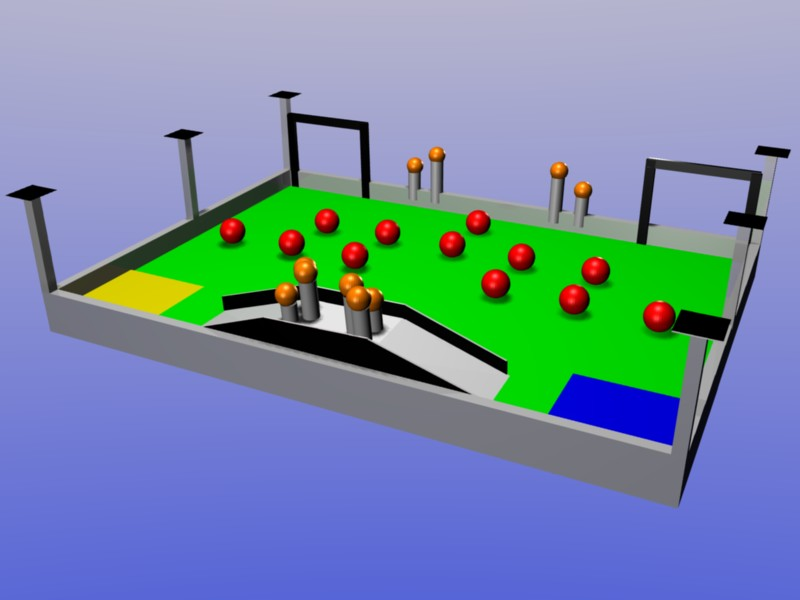
\includegraphics[width=.7\linewidth]{concours_robotique}
\end{center}
\end{frame}


\end{document}
